\documentclass{beamer}
\usepackage{lmodern}
\usepackage{etex}
\usepackage[utf8]{inputenc}
\usepackage[T1]{fontenc}
\usepackage[english]{babel}
\usepackage{amssymb}
\usepackage{epsfig,shadow}
\usepackage{verbatim}
\usepackage{pstricks}
\usepackage{beamerthemesplit}
\usepackage{graphicx}
\usepackage{comment}
\usepackage{algorithm}
\usepackage{listings}
\usepackage{figlatex}
\usepackage{algorithmic}
\usepackage{multirow}

\graphicspath{{fig/}{campagne/fig}}
\newcommand{\talk}[2]{{#1} dit : {#2}}
\newcommand{\erik}[1]{\talk{Erik}{#1}}
\newcommand{\brice}[1]{\talk{Brice}{#1}}
\beamertemplatetransparentcovereddynamic

%\setbeamertemplate{background canvas}[vertical shading][bottom=red!10,top=blue!10]
%\usetheme{Warsaw}

\usecolortheme{progressbar}
\usefonttheme{progressbar}
\useoutertheme{progressbar}
\useinnertheme{progressbar}

\newcommand{\bordereau}{Bordereau\xspace}
\newcommand{\genepi}{Genepi\xspace}
\newcommand{\minelement}{{\em min\_element}\xspace}
\newcommand{\stablesort}{{\em stable\_sort}\xspace}
\newcommand{\merge}{{\em merge}\xspace}
\newcommand{\sort}{{\em sort}\xspace}
\newcommand{\find}{{\em find}\xspace}
\setbeamertemplate{navigation symbols}{}
\beamertemplatetransparentcovereddynamic
\newcommand{\pastel}{PaSTeL\xspace}

\definecolor{javared}{rgb}{0.6,0,0} % for strings
\definecolor{javagreen}{rgb}{0.25,0.5,0.35} % comments
\definecolor{javapurple}{rgb}{0.5,0,0.35} % keywords
\definecolor{javadocblue}{rgb}{0.25,0.35,0.75} % java


\lstdefinestyle{BOAST}{
  language=Ruby,
  basicstyle=\tiny\ttfamily,
  keywordstyle=\color{javapurple}\bfseries,
  stringstyle=\color{javared},
  commentstyle=\color{javagreen},
  backgroundcolor=\color{white},
  morekeywords={BOAST, pr, decl, opn, close}
}

\title{BOAST}
\subtitle{Using BOAST: an Introduction }
\author{Brice Videau\\
(LIG - NANOSIM)}

\date{\textbf{BOAST Tutorial}\\September 19, 2014}

\begin{document}

\frame{\titlepage}

\section{Installing BOAST}


\begin{frame}[fragile]

    \frametitle{Installing BOAST}

Install ruby, version >= 1.9.3\\
On recent debian-based distributions:
\lstset{language=Bash,
basicstyle=\ttfamily,
keywordstyle=\color{javapurple}\bfseries,
stringstyle=\color{javared},
commentstyle=\color{javagreen},
numbers=left,
tabsize=4,
showspaces=false,
showstringspaces=false}
\begin{lstlisting}
sudo apt-get install ruby ruby-dev
\end{lstlisting}
And then install the BOAST gem (ruby module):
\begin{lstlisting}
sudo gem install BOAST
\end{lstlisting}
If on a cluster frontend:
\begin{lstlisting}
gem install --user-install BOAST
\end{lstlisting}

\end{frame}

\section{First Steps}

\begin{frame}[fragile]
\frametitle{First interactive steps}
\lstset{language=Bash,
basicstyle=\ttfamily,
keywordstyle=\color{javapurple}\bfseries,
stringstyle=\color{javared},
commentstyle=\color{javagreen},
numbers=left,
tabsize=4,
showspaces=false,
showstringspaces=false}
Interactive Ruby:
\begin{lstlisting}
irb
\end{lstlisting}
Simple BOAST commands:
\lstset{style=BOAST}
\begin{lstlisting}
irb(main):001:0> require 'BOAST'
=> true
irb(main):002:0> a = BOAST::Int "a"
=> a
irb(main):003:0> b = BOAST::Real "b"
=> b
irb(main):004:0> BOAST::decl a, b
integer(kind=4) :: a
real(kind=8) :: b
=> [a, b]
\end{lstlisting}
\end{frame}

\begin{frame}[fragile]
\frametitle{Defining a Procedure}
Simple BOAST Procedure:
\lstset{style=BOAST}
\footnotesize
\begin{lstlisting}
05:0> p = BOAST::Procedure( "test_proc", [a,b] )
06:0> BOAST::opn p
SUBROUTINE test_proc(a, b)
  integer, parameter :: wp=kind(1.0d0)
  integer(kind=4) :: a
  real(kind=8) :: b
007:0> BOAST::lang = BOAST::C
008:0> BOAST::opn p
void test_proc(int32_t a, double b){
009:0> BOAST::close p
}
\end{lstlisting}
Available languages are FORTRAN, C, CUDA, CL (OpenCL)
\end{frame}

\begin{frame}[fragile]
\frametitle{Defining a Full Procedure:}
\lstset{style=BOAST}
\tiny
\begin{lstlisting}
010:0> a = BOAST::Real( "a", :dir => :in)
011:0> b = BOAST::Real( "b", :dir => :out)
012:0> p = BOAST::Procedure( "test_proc", [a,b] ) {
012:1>   BOAST::pr b === a + 2
012:2> }
013:0> BOAST::lang = BOAST::FORTRAN
014:0> BOAST::pr p
SUBROUTINE test_proc(a, b)
    integer, parameter :: wp=kind(1.0d0)
    real(kind=8), intent(in) :: a
    real(kind=8), intent(out) :: b
    b = a + 2
END SUBROUTINE test_proc
\end{lstlisting}
\end{frame}

\begin{frame}[fragile]
\frametitle{Creating a Computing Kernel}
\lstset{style=BOAST}
\tiny
\begin{lstlisting}
n = BOAST::Int(  "n", :dir => :in )
a = BOAST::Real( "a", :dir => :in,  :dim => [BOAST::Dim(n)] )
b = BOAST::Real( "b", :dir => :out, :dim => [BOAST::Dim(n)] )
p = BOAST::Procedure( "test_proc", [n, a, b] ) {
  BOAST::decl i = BOAST::Int( "i" )
  BOAST::pr BOAST::For( i, 1, n ) {
    BOAST::pr b[i] === a[i] + 2
  }
}
k = BOAST::CKernel::new
BOAST::pr p
k.procedure = p
k.build
BOAST::verbose = true
k.build
> gcc -O2 -Wall -fPIC -I/usr/lib/ruby/1.9.1/x86_64-linux -I/usr/include/ruby-1.9.1 -I/usr/include/ruby-1.9.1/x86_64-linux -I/var/lib/gems/1.9.1/gems/narray-0.6.0.9 -DHAVE_NARRAY_H -c -o /tmp/Mod_test_proc20140624_19378_1qdep6u.o /tmp/Mod_test_proc20140624_19378_1qdep6u.c
> gfortran -O2 -Wall -fPIC -c -o /tmp/test_proc20140624-19378-1qdep6u.o /tmp/test_proc20140624-19378-1qdep6u.f90
> gcc -shared -o /tmp/Mod_test_proc20140624_19378_1qdep6u.so /tmp/Mod_test_proc20140624_19378_1qdep6u.o /tmp/test_proc20140624-19378-1qdep6u.o -Wl,-Bsymbolic-functions -Wl,-z,relro -rdynamic -Wl,-export-dynamic -L/usr/lib -lruby-1.9.1 -lrt
\end{lstlisting}
\end{frame}

\begin{frame}[fragile]
\frametitle{Running a Computing Kernel}
\lstset{style=BOAST}
\tiny
\begin{lstlisting}
require 'narray'
n = BOAST::Int(  "n", :dir => :in )
a = BOAST::Real( "a", :dir => :in,  :dim => [BOAST::Dim(n)] )
b = BOAST::Real( "b", :dir => :out, :dim => [BOAST::Dim(n)] )
p = BOAST::Procedure( "test_proc", [n, a, b] ) {
  BOAST::decl i = BOAST::Int( "i" )
  BOAST::pr BOAST::For( i, 1, n ) {
    BOAST::pr b[i] === a[i] + 2
  }
}
k = BOAST::CKernel::new
BOAST::pr p
k.procedure = p

input  = NArray.float(1024).random
output = NArray.float(1024)
k.run(input.length, input, output)
(output - input).each { |val|
  raise "Error!" if (val-2).abs > 1e-15
}
stats = k.run(input.length, input, output)
puts "#{stats[:duration]} s"
> 4.911e-06 s
\end{lstlisting}
\end{frame}

\section{BOAST Samples}
\begin{frame}
\frametitle{BOAST Samples}

\end{frame}

\subsection{The Canonic Case}
\begin{frame}[fragile]
\frametitle{The Canonic Case: Vector Addition Kernel}
\tiny
\lstset{style=BOAST}
\begin{lstlisting}
def BOAST::vector_add
  kernel = CKernel::new
  function_name = "vector_add"
  n = Int("n",{:dir => :in, :signed => false})
  a = Real("a",{:dir => :in, :dim => [ Dim(0,n-1)] })
  b = Real("b",{:dir => :in, :dim => [ Dim(0,n-1)] })
  c = Real("c",{:dir => :out, :dim => [ Dim(0,n-1)] })
  i = Int("i",{:signed => false})
  pr p = Procedure(function_name, [n,a,b,c]) {
    decl i
    if [CL, CUDA].include?(get_lang) then
      pr i === get_global_id(0)
      pr c[i] === a[i] + b[i]
    else
      pr For(i,0,n-1) {
        pr c[i] === a[i] + b[i]
      }
    end
  }
  kernel.procedure = p
  return kernel
end
\end{lstlisting}
\end{frame}

\begin{frame}[fragile]
\frametitle{Running the Kernel}
\lstset{style=BOAST}
\tiny
\begin{lstlisting}
n = 1024*1024
a = NArray.sfloat(n).random
b = NArray.sfloat(n).random
c = NArray.sfloat(n)

epsilon = 10e-15

c_ref = a + b

[:FORTRAN, :C, :CL, :CUDA].each { |l|
  set_lang( BOAST.const_get(l)  )
  puts "#{l}:"
  k = vector_add
  puts k.print
  c.random!
  k.run(n, a, b, c, :global_work_size => [n,1,1], :local_work_size => [32,1,1])
  diff = (c_ref - c).abs
  diff.each { |elem|
    raise "Warning: residue too big: #{elem}" if elem > epsilon
  }
}
puts "Success!"
\end{lstlisting}
\end{frame}
\subsection{Building Kernels}
\begin{frame}[fragile]
\frametitle{Building Kernels}
\begin{itemize}
\item Running a kernel builds it (if it is not already built).
\item Kernels can be built beforehand.
\item Usual build parameters can be specified.
\end{itemize}
Sample:
\lstset{style=BOAST}
\tiny
\begin{lstlisting}
  k.build({:FC => 'gfortran', :CC => 'gcc',\
           :FCFLAGS => "-O2", :LDFLAGS => ""})
  k.build({:FC => 'gfortran', :CC => 'gcc',\
           :FCFLAGS => "-O2 -fopenmp",:LDFLAGS => "-fopenmp"})
  k.build({:FC => 'ifort',    :CC => 'icc',
           :FCFLAGS => "-O2 -openmp" ,:LDFLAGS => "-openmp",:LD => "ifort"})
\end{lstlisting}
\normalsize
\begin{itemize}
\item Probes can be inserted at compile time.
\item Default: high resolution timer.
\end{itemize}
\lstset{style=BOAST}
\tiny
\begin{lstlisting}
  stats = k.run(...)
  puts stats[:duration]+" s"
\end{lstlisting}
\end{frame}

\subsection{Real Life Examples}
\begin{frame}
\frametitle {Real Life Examples}
\end{frame}

\begin{frame}[fragile]
\frametitle{SPECFEM3D assemble\_boundary\_potential\_on\_device : Reference}
\tiny
\lstset{language=C,
basicstyle=\ttfamily,
keywordstyle=\color{javapurple}\bfseries,
stringstyle=\color{javared},
commentstyle=\color{javagreen},
numbers=left,
tabsize=4,
showspaces=false,
showstringspaces=false}
\begin{lstlisting}
typedef float realw;
__global__ void assemble_boundary_potential_on_device(realw* d_potential_dot_dot_acoustic,
                                                      realw* d_send_potential_dot_dot_buffer,
                                                      int num_interfaces,
                                                      int max_nibool_interfaces,
                                                      int* d_nibool_interfaces,
                                                      int* d_ibool_interfaces) {

  int id = threadIdx.x + blockIdx.x*blockDim.x + blockIdx.y*gridDim.x*blockDim.x;
  int iglob,iloc;

  for( int iinterface=0; iinterface < num_interfaces; iinterface++) {
    if(id < d_nibool_interfaces[iinterface]) {

      iloc = id + max_nibool_interfaces*iinterface;

      iglob = d_ibool_interfaces[iloc] - 1;

      // assembles values
      atomicAdd(&d_potential_dot_dot_acoustic[iglob],d_send_potential_dot_dot_buffer[iloc]);
    }
  }
}
\end{lstlisting}

\end{frame}

\begin{frame}[fragile]
\frametitle{SPECFEM3D assemble\_boundary\_potential\_on\_device : BOAST (1)}
\lstset{style=BOAST}
\tiny
\begin{lstlisting}
def BOAST::assemble_boundary_potential_on_device(ref = true)
  push_env( :array_start => 0 )
  kernel = CKernel::new
  function_name = "assemble_boundary_potential_on_device"
  num_interfaces                  = Int("num_interfaces",                   \
                                        :dir => :in)
  max_nibool_interfaces           = Int("max_nibool_interfaces",            \
                                        :dir => :in)
  d_potential_dot_dot_acoustic    = Real("d_potential_dot_dot_acoustic",    \
                                        :dir => :out,:dim => [ Dim() ])
  d_send_potential_dot_dot_buffer = Real("d_send_potential_dot_dot_buffer", \
                                        :dir => :in, :dim => [ Dim(num_interfaces*max_nibool_interfaces) ])
  d_nibool_interfaces             = Int("d_nibool_interfaces",              \
                                        :dir => :in, :dim => [ Dim(num_interfaces) ])
  d_ibool_interfaces              = Int("d_ibool_interfaces",               \
                                        :dir => :in, :dim => [ Dim(num_interfaces*max_nibool_interfaces) ])
  p = Procedure(function_name, [d_potential_dot_dot_acoustic,d_send_potential_dot_dot_buffer,num_interfaces,max_nibool_interfaces,d_nibool_interfaces,d_ibool_interfaces])
\end{lstlisting}

\end{frame}

\begin{frame}[fragile]
\frametitle{SPECFEM3D assemble\_boundary\_potential\_on\_device : BOAST (2)}
\lstset{style=BOAST}
\tiny
\begin{lstlisting}
  if(get_lang == CUDA and ref) then
    @@output.print File::read("specfem3D/#{function_name}.cu")
  elsif(get_lang == CUDA or get_lang == CL) then
    opn p
    id         = Int("id")
    iglob      = Int("iglob")
    iloc       = Int("iloc")
    iinterface = Int("iinterface")
    decl id, iglob, iloc, iinterface
    pr id === get_global_id(0) + get_global_size(0)*get_global_id(1)
    pr For(iinterface, 0, num_interfaces-1) {
      pr If(id<d_nibool_interfaces[iinterface]) {
        pr iloc === id + max_nibool_interfaces*iinterface
        pr iglob === d_ibool_interfaces[iloc] - 1
        pr atomicAdd(d_potential_dot_dot_acoustic + iglob, \
                     d_send_potential_dot_dot_buffer[iloc])
      }
    }
    close p
  else
    raise "Unsupported language!"
  end
  pop_env( :array_start )
  kernel.procedure = p
  return kernel
end
\end{lstlisting}

\end{frame}


\begin{frame}[fragile]
\frametitle{SPECFEM3D assemble\_boundary\_potential\_on\_device : Generated CUDA}
\tiny
\lstset{language=C,
basicstyle=\ttfamily,
keywordstyle=\color{javapurple}\bfseries,
stringstyle=\color{javared},
commentstyle=\color{javagreen},
numbers=left,
tabsize=4,
showspaces=false,
showstringspaces=false}
\begin{lstlisting}
__global__ void assemble_boundary_potential_on_device(float * d_potential_dot_dot_acoustic, const float * d_send_potential_dot_dot_buffer, const int num_interfaces, const int max_nibool_interfaces, const int * d_nibool_interfaces, const int * d_ibool_interfaces){
  int id;
  int iglob;
  int iloc;
  int iinterface;
  id = threadIdx.x + ((blockIdx.x) * (blockDim.x)) + (((gridDim.x) * (blockDim.x)) * (threadIdx.y + ((blockIdx.y) * (blockDim.y))));
  for(iinterface=0; iinterface<=num_interfaces - (1); iinterface+=1){
    if(id < d_nibool_interfaces[iinterface - 0]){
      iloc = id + ((max_nibool_interfaces) * (iinterface));
      iglob = d_ibool_interfaces[iloc - 0] - (1);
      atomicAdd(d_potential_dot_dot_acoustic + (iglob), d_send_potential_dot_dot_buffer[iloc - 0]);
    }
  }
}
\end{lstlisting}

\end{frame}

\begin{frame}[fragile]
\frametitle{SPECFEM3D assemble\_boundary\_potential\_on\_device : Generated OpenCL}
\tiny
\lstset{language=C,
basicstyle=\ttfamily,
keywordstyle=\color{javapurple}\bfseries,
stringstyle=\color{javared},
commentstyle=\color{javagreen},
numbers=left,
tabsize=4,
showspaces=false,
showstringspaces=false}
\begin{lstlisting}

__kernel void assemble_boundary_potential_on_device(__global float * d_potential_dot_dot_acoustic, const __global float * d_send_potential_dot_dot_buffer, const int num_interfaces, const int max_nibool_interfaces, const __global int * d_nibool_interfaces, const __global int * d_ibool_interfaces){
  int id;
  int iglob;
  int iloc;
  int iinterface;
  id = get_global_id(0) + ((get_global_size(0)) * (get_global_id(1)));
  for(iinterface=0; iinterface<=num_interfaces - (1); iinterface+=1){
    if(id < d_nibool_interfaces[iinterface - 0]){
      iloc = id + ((max_nibool_interfaces) * (iinterface));
      iglob = d_ibool_interfaces[iloc - 0] - (1);
      atomicAdd(d_potential_dot_dot_acoustic + (iglob), d_send_potential_dot_dot_buffer[iloc - 0]);
    }
  }
}
\end{lstlisting}
\end{frame}
%\begin{frame}
%\frametitle{BigDFT Synthesis Kernel}
%\centering 
%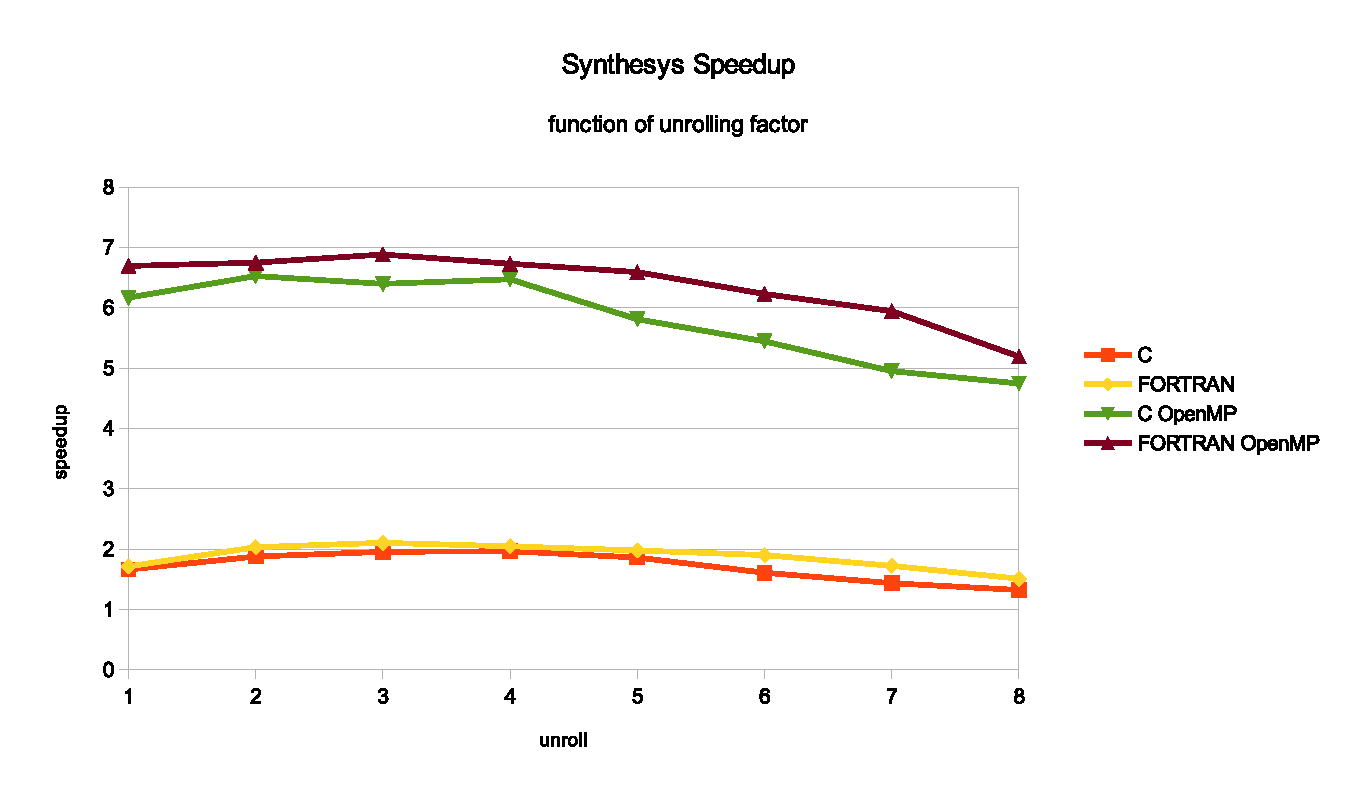
\includegraphics[scale=0.5]{Res_synthesis}\\
%
%
%\end{frame}




\end{document}
